% Carattere dimensione 12
\documentclass[12pt]{report}

% Per la stampa fronte-retro sostituire con:
% \documentclass[12pt, twoside]{report}

% Margini (4cm a sx, 2.5cm a dx, 2.5cm in alto, 2.5cm in basso)
\usepackage[top=2.5cm, bottom=2.5cm, left=4cm, right=2.5cm, centering]{geometry}

% Per la stampa fronte-retro sostituire con: 
% \usepackage[top=2.5cm, bottom=2.5cm, inner=4cm, outer=4cm, right=2.5cm, centering]{geometry}

% Interlinea
\linespread{1.5}

% Librerie utili
\usepackage[italian]{babel} % applicazione regole di scrittura per la lingua italiana 
\usepackage[utf8]{inputenc} % codifica UTF-8
\usepackage{scrlayer-scrpage} % stili pagina per il frontespizio
\ifoot[]{}
\cfoot[]{}
\ofoot[\pagemark]{\pagemark}
\pagestyle{scrplain}
\usepackage{mathptmx} % font Times New Roman (simile)
\usepackage{graphicx} % inserimento di immagini
\usepackage{csquotes} % per le citazioni "in blocco"
\usepackage[backend=biber, sorting=none, ]{biblatex} % bibliografia con pacchetto biblatex (https://ctan.org/pkg/biblatex?lang=en)
\addbibresource{bibliography.bib}
\appto{\bibsetup}{\raggedright}

\usepackage{titlesec} % per la formattazione dei titoli delle sezioni, capitoli etc.
\usepackage{float} % per il posizionamento delle immagini

\usepackage{listings} % per il codice di programmazione
% Fonte https://en.wikibooks.org/wiki/LaTeX/Source_Code_Listings. Per la lista di sintassi riconosciute.
\renewcommand{\lstlistingname}{Code}% Listing -> Codice
\usepackage{xcolor}  % stile del codice
\definecolor{mygreen}{rgb}{0,0.6,0}
\definecolor{mygray}{rgb}{0.5,0.5,0.5}
\definecolor{mymauve}{rgb}{0.58,0,0.82}
\definecolor{darkgray}{rgb}{.4,.4,.4}
\definecolor{navy}{HTML}{000080}
\definecolor{purple}{rgb}{0.65, 0.12, 0.82}
\definecolor{codepurple}{rgb}{0.58,0,0.82}
\definecolor{backcolour}{rgb}{0.95,0.95,0.92}

% \usepackage{longtable}
\usepackage{tabularx}


% Stili configurabili del codice (lslisting) 
\lstset{ %
belowcaptionskip=0.5em,
backgroundcolor=\color{backcolour}, % choose the background color; you must add \usepackage{color} or \usepackage{xcolor}
basicstyle=\footnotesize, % the size of the fonts that are used for the code
breakatwhitespace=false, % sets if automatic breaks should only happen at whitespace
breaklines=true, % sets automatic line breaking
captionpos=b, % sets the caption-position to bottom
commentstyle=\color{mygreen}, % comment style
deletekeywords={...}, % if you want to delete keywords from the given language
escapeinside={\%*}{*)}, % if you want to add LaTeX within your code
extendedchars=true, % lets you use non-ASCII characters; for 8-bits encodings only, does not work with UTF-8
frame=single, % adds a frame around the code
keepspaces=true, % keeps spaces in text, useful for keeping indentation of code (possibly needs columns=flexible)
keywordstyle=\color{codepurple}, % keyword style
% language=Octave, % the language of the code
morekeywords={*,...}, % if you want to add more keywords to the set
numbers=left, % where to put the line-numbers; possible values are (none, left, right)
numbersep=5pt, % how far the line-numbers are from the code
numberstyle=\tiny\color{mygray}, % the style that is used for the line-numbers
rulecolor=\color{black}, % if not set, the frame-color may be changed on line-breaks within not-black text (e.g. comments (green here))
showspaces=false, % show spaces everywhere adding particular underscores; it overrides 'showstringspaces'
showstringspaces=false, % underline spaces within strings only
showtabs=false, % show tabs within strings adding particular underscores
stepnumber=1, % the step between two line-numbers. If it's 1, each line will be numbered
stringstyle=\color{mymauve}, % string literal style
tabsize=2, % sets default tabsize to 2 spaces
title=\lstname % show the filename of files included with \lstinputlisting; also try caption instead of title
}


\setlength{\parindent}{0pt}


% END of listing package 

% Formato delle intestazioni
\titleformat{\chapter}[block]
  {\normalfont\LARGE\bfseries}{\thechapter.}{0.5em}{\LARGE}
\titlespacing*{\chapter}{0pt}{-20pt}{25pt}

\begin{document}

% Frontespizio
\begin{titlepage}
% \begin{figure}
%     \centering\includegraphics[scale=0.5]{immagini/cherubino_pant541.png}
% \end{figure}

\begin{center}
    {\LARGE{ Emotion Detection on song lyrics stanzas \\}}
    \vspace{3cm}
    {\Large { TEXT ANALYTICS }}\\
    \vspace{1.5cm}
    {\Large { Group 2 }}\\
    \vspace{1.5cm}
    {\Large { Barbieri, Bosco, Ferrara, Rotellini, Zizza }}
\end{center}

% \centering{\large{\bf ANNO ACCADEMICO 20xx/20xx }}
\end{titlepage}
% Fine frontespizio

\renewcommand{\contentsname}{Index}
\tableofcontents
\thispagestyle{empty}


\renewcommand{\listfigurename}{List of figures}
\listoffigures

\thispagestyle{empty}
\clearpage
\setcounter{page}{1}
\addtocontents{toc}{\protect\thispagestyle{empty}}
\addcontentsline{toc}{chapter}{Introduction} % Capitolo non numerato
\chapter*{Introduction}
\label{ch:Introduction}
Lyrics serve as one of the main foundations of songs, playing a crucial role in
expressing feelings in many different ways.
The emotional tone of songs can serve various purposes, such as
automatized playlist creation or songs' organization,
offering an alternative to the more traditional genre-based classification. \\
%Analyzing the emotional tone of song texts can give useful insights about individual mental states, cultural trends, social issues and more.
% The main goal of this project is to perform emotion detection on stanzas of songs.
% The goal of this project is the development of 4 Machine Learning models
% that perform emotion detection on songs' stanzas.
To obtain a deeper understanding of emotional fluctuations within the texts,
the models assign emotion labels to individual stanzas instead of full songs.
The emotion labels correspond to Robert Plutchik's eight primary emotions
(shown in figure~\ref{fig:primary_emotions}), providing a comprehensive range
for representing various emotional states.\\
\begin{figure}[H]
    \centering
    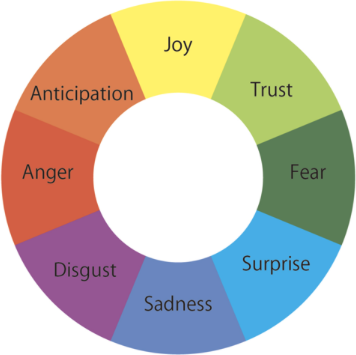
\includegraphics[scale= 0.25]{pictures/plutchik_primary_emotions.png}
    \caption{Plutchik's eight primary emotions}
    \label{fig:primary_emotions}
\end{figure}

This report aims to clearly cover and illustrate various aspects of the work. 
The \textit{Methods} chapter contains a detailed explanation of the data and
procedures used in the project, providing descriptions of each part implemented
in the project.
The \textit{Results} chapter presents an overview of the
obtained outcomes.
These results are further explored in the final sections, \textit{Discussion}
and \textit{Conclusions}, which interpret the general findings, recap the
primary objectives of the work, and discuss the importance or potential
applications of the results.

\clearpage

% Dataset overview
% !!! cut, content in intro
% % !!!
% cut at the moment; content moved to introduction

\chapter{Dataset overview}
\label{ch:capitolo1}

% copy-pasted from project proposal
The dataset utilized in this project represents a subset of songs
derived from the Genius Song Lyrics Dataset\textsuperscript{\cite{geniusdataset}}.
The dataset contains 11 attributes
that represent various song data, including the lyrics.
The original dataset includes songs in all languages: for our aim
we will be using the english ones only.\\

The dataset doesn't have emotion labels, which are essential for training the models.
To create the ground truth, the model
Albert Base v2\textsuperscript{\cite{albert-base-v2}} was used, classifying
stanzas' lyrics with Plutchik's eight primary emotions.

% The stanzas are labeled using Robert Plutchik's 8 primary emotions;
% the emotions included in this representation are:
% anger, fear, sadness, disgust, surprise, anticipation, trust, and joy.
% Such multifaceted emotions allow us to finely analyze the feelings and
% moods conveyed by songs.
% 
% \clearpage

% Preprocessing
\chapter{Preprocessing}
\label{ch:capitolo2}

The first step in the preprocessing phase involved sampling the original dataset while preserving the original proportions of the different genres. 
This ensured that the genre distribution in the subset remained representative of the full dataset.


\clearpage

% static models
\chapter{Static Models}
\label{ch:static_models}


\section{Random Forest}

\section{SVM}


\clearpage

% neural networks
\chapter{Neural Networks}
\label{ch:capitolo4}

\section{One-Dimensional Convolutional Neural Network}

\section{Recurrent Neural Network}

\clearpage

\addcontentsline{toc}{chapter}{Key findings and conclusions} % Capitolo non numerato
\chapter*{Key findings and conclusions}
\label{ch:conclusioni}
\clearpage

% \renewcommand{\contentsname}{Bibliography}
% \bibliographystyle{plain} % We choose the "plain" reference style
% \bibliography{bibliography} % Entries are in the refs.bib file
% \addbibresource{bibliography.bib}
\printbibliography

\end{document}